\documentclass[ucs,10pt]{beamer}

\usepackage{color}
\usepackage{url}
\usepackage{algorithmic}
\usepackage{amsmath}
\usepackage{amssymb}
\usepackage{amsxtra}
\usepackage{graphicx}
\usepackage{tikz}
\usetikzlibrary{shapes.geometric}


\usepackage{listings}
\lstset{language=C++,
    basicstyle=\footnotesize,
    numberstyle=\tiny,
    showstringspaces=false,
    numbers=left,
    frame=none,
    commentstyle=\color{purple},
    captionpos=t
  }

% Template for talks using the Logo of STCE and Corporate Design of RWTH Aachen
% adapted from:
% https://www.mi.fu-berlin.de/w/Mi/BeamerTemplateCorporateDesign

\usepackage{amsmath,dsfont,listings}

%%% STCE logo
% small version for upper right corner of normal pages
\pgfdeclareimage[height=0.9cm]{university-logo}{logo.png}
\logo{\pgfuseimage{university-logo}}
% large version for upper right corner of title page
\pgfdeclareimage[height=1cm]{big-university-logo}{logo.png}
\newcommand{\titleimage}[1]{\pgfdeclareimage[height=2cm]{title-image}{#1}}
\titlegraphic{\pgfuseimage{title-image}}
%%% end STCE logo

% NOTE: 1cm = 0.393 in = 28.346 pt;    1 pt = 1/72 in = 0.0352 cm
\setbeamersize{text margin right=3.5mm, text margin left=7.5mm}  % text margin

% colors to be used
\definecolor{text-grey}{RGB}{51, 51, 51} % grey text on white background
\definecolor{bg-grey}{rgb}{0.66, 0.65, 0.60} % grey background (for white text)
\definecolor{rwth-blue}{RGB}{0, 83, 159} % blue text
\definecolor{rwth-green}{RGB}{153, 204, 0} % green text
\definecolor{rwth-red}{RGB}{204, 0, 0} % red text (used by \alert)

\definecolor{rwth-blue-2}{RGB}{64,127,183}
\definecolor{rwth-blue-3}{RGB}{142,186,229}
\definecolor{rwth-blue-4}{RGB}{199,221,242}
\definecolor{rwth-blue-5}{RGB}{232,241,250}

% switch off the sidebars
% TODO: loading \useoutertheme{sidebar} (which is maybe wanted) also inserts
%   a sidebar on title page (unwanted), also indents the page title (unwanted?),
%   and duplicates the navigation symbols (unwanted)
\setbeamersize{sidebar width left=0cm, sidebar width right=0mm}
\setbeamertemplate{sidebar right}{}
\setbeamertemplate{sidebar left}{}
%    XOR
% \useoutertheme{sidebar}

% frame title
% is truncated before logo and splits on two lines
% if neccessary (or manually using \\)
\setbeamertemplate{frametitle}{%
    \vskip-35pt 
\color{black}\normalsize%
    \begin{minipage}[b][23pt]{\linewidth}%
    \flushleft\insertframetitle%
    \end{minipage} \\
\vskip-4pt
\color{rwth-blue}\rule{\textwidth}{0.4pt}
}

%%% title page
% TODO: get rid of the navigation symbols on the title page.
%   actually, \frame[plain] *should* remove them...
\setbeamertemplate{title page}{
% upper right: STCE logo
\vskip2pt\hfill \pgfuseimage{big-university-logo} \\
\vfill
\vskip6pt\hskip3pt
% title image of the presentation
% set the title and the author
\begin{center}
\vskip4pt
\large \inserttitle \vskip5pt  \small \insertsubtitle
\vskip8pt
	\normalsize \insertauthor  
\vskip8pt
%	\includegraphics[width=2cm]{utils/foto_naumann}	
%\\ [-3mm]
	\footnotesize \insertinstitute 
\end{center}
\vfill
}
%%% end title page

%%% colors
\usecolortheme{lily}
\setbeamercolor*{normal text}{fg=black,bg=white}
\setbeamercolor*{alerted text}{fg=rwth-red}
\setbeamercolor*{example text}{fg=rwth-green}
\setbeamercolor*{structure}{fg=black}

\setbeamercolor*{block title}{fg=white,bg=black!50}
\setbeamercolor*{block title alerted}{fg=white,bg=black!50}
\setbeamercolor*{block title example}{fg=white,bg=black!50}

\setbeamercolor*{block body}{bg=black!10}
\setbeamercolor*{block body alerted}{bg=black!10}
\setbeamercolor*{block body example}{bg=black!10}

\setbeamercolor{bibliography entry author}{fg=black}
% TODO: this doesn't work at all:
\setbeamercolor{bibliography entry journal}{fg=text-grey}

\setbeamercolor{item}{fg=black}
\setbeamercolor{navigation symbols}{fg=text-grey,bg=bg-grey}
%%% end colors

%%% headline
\setbeamertemplate{headline}{
\vskip10pt \hfill\insertlogo\hspace{3.5mm} % logo on the right
%\vskip0pt\color{rwth-blue}\rule{\textwidth}{0.4pt} % horizontal line
}
%%%% end headline

%%% footline
\newcommand{\footlinetext}{\insertshortinstitute, \insertshorttitle}
\setbeamertemplate{footline}{
\vskip5pt\color{rwth-blue}\rule{\textwidth}{0.4pt}\\ % horizontal line
\vskip2pt
\makebox[123mm]{\hspace{7.5mm}
\color{black}\footlinetext
%\hfill \raisebox{-1pt}{\usebeamertemplate***{navigation symbols}}
\hfill \insertframenumber}
\vskip4pt
}
%%% end footline

%%% settings for listings package
\lstset{extendedchars=true, showstringspaces=false, basicstyle=\footnotesize\sffamily, tabsize=2, breaklines=true, breakindent=10pt, frame=l, columns=fullflexible}
\lstset{language=C++} % this sets the syntax highlighting
\lstset{mathescape=true} % this switches on $...$ substitution in code
% enables UTF-8 in source code:
\lstset{literate={ä}{{\"a}}1 {ö}{{\"o}}1 {ü}{{\"u}}1 {Ä}{{\"A}}1 {Ö}{{\"O}}1 {Ü}{{\"U}}1 {ß}{\ss}1}
%%% end listings
  

\AtBeginSection[]
{
  \begin{frame}<beamer>{Outline}
    \tableofcontents[currentsection,currentsubsection]
  \end{frame}
}

\newcommand\inc{{\small \;\mathrel{+\!\!=}\;}}
\newcommand\dec{{\small \;\mathrel{-\!\!=}\;}}
\newcommand\ERT{{\footnotesize \textsc{Ert}}}
\newcommand\MEM{{\footnotesize \textsc{Mem}}}
\newcommand\OPS{{\footnotesize \textsc{Ops}}}
\newcommand\RSS{{\footnotesize \textsc{Rss}}}
\newcommand{\dollar}{\mbox{\textdollar}}
\newcommand{\pe}{\mathrel{+}=}
\newcommand{\ass}{\mathrel{:}=}
\newcommand{\A}{{\bf a}}
\newcommand{\C}{{\bf c}}
\newcommand{\B}{{\bf b}}
\renewcommand{\r}{{\bf r}}
\newcommand{\X}{{\bf x}}
\newcommand{\tx}{\tilde{x}}
\newcommand{\dx}{\Delta x}
\newcommand{\Y}{{\bf y}}
\newcommand{\Z}{{\bf z}}
\newcommand{\V}{{\bf v}}
\newcommand{\U}{{\bf u}}
\renewcommand{\P}{{\bf p}}
\newcommand{\R}{{\mathbb{R}}}
\newcommand{\Kappa}{{\cal K}}
\newcommand{\fma}{{\small {\tt fma}}}

\begin{document}
\title[AD2024, Chicago, Sep 16-19, 2024]{{\bf An Efficient Local Optimizer-Tracking Solver for Differential-Algebriac Equations with Optimization Criteria}}
\author[]{Alexander Fleming\footnote{\scriptsize fleming@stce.rwth-aachen.de} \and Jens Deussen \and Uwe Naumann}
\institute[STCE]{\underline{S}oftware and \underline{T}ools for \underline{C}omputational \underline{E}ngineering\footnote{\scriptsize https://www.stce.rwth-aachen.de/} \vspace{1mm} \\ RWTH Aachen, Germany \vspace{5mm} \\ 
8th International Conference on Algorithmic Differentiation (AD2024)
}
		
\begin{frame}[plain]
\titlepage
\end{frame}

\begin{frame}
	\frametitle{Contents}
\tableofcontents
\end{frame}

\section{Motivation}

\begin{frame}
\frametitle{Motivation}
\vfill
	\begin{minipage}[c]{.6\linewidth}
Let a differentiable program
\vfill
$$
\Y=F(\X) : \R^n \rightarrow \R^m
$$
\vfill
decompose as
\vfill
	\color{rwth-blue}
$$
F=F_q \circ F_{q-1} \circ \ldots \circ F_2 \circ F_1
$$
	\color{black}
\vfill
with elemental functions $F_i,$ such that 
\vfill
	$$\Z_i=F_i(\Z_{i-1}) : \R^{n_i} \rightarrow \R^{m_i} \; ,$$ 
\vfill
	for $i=1,\ldots,q$
and $\Z_0=\X,$ $\Y=\Z_q.$
	\end{minipage}
	\begin{minipage}[c]{.35\linewidth}
		Sample \textcolor{rwth-blue}{tape} (DAG): \vspace{3mm} \\
		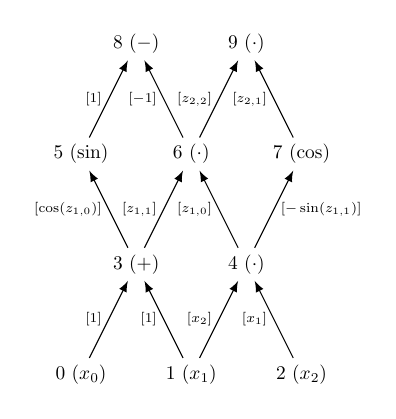
\begin{tikzpicture}[scale=.7, transform shape]
  \begin{pgfscope}
    \tikzstyle{every node}=[]
          \node (1) at (0,0) {$0~(x_0)$};
          \node (2) at (2,0) {$1~(x_1)$};
          \node (3) at (4,0) {$2~(x_2)$};
          \node (4) at (1,2) {$3~(+)$};
          \node (5) at (3,2) {$4~(\cdot)$};
          \node (6) at (0,4) {$5~(\sin)$};
          \node (7) at (2,4) {$6~(\cdot)$};
          \node (8) at (4,4) {$7~(\cos)$};
          \node (9) at (1,6) {$8~(-)$};
          \node (10) at (3,6) {$9~(\cdot)$};
  \end{pgfscope}
  \begin{scope}[-latex]
          \draw (1) -- (4) node[midway, left] {\scriptsize $\left [1 \right ]$};
          \draw (2) -- (4) node[midway, left] {\scriptsize $\left [1 \right ]$};
          \draw (2) -- (5) node[midway, left] {\scriptsize $\left [x_2 \right ]$};
          \draw (3) -- (5) node[midway, left] {\scriptsize $\left [x_1 \right ]$};
          \draw (4) -- (6) node[midway, left] {\scriptsize $\left [\cos(z_{1,0}) \right ]$};
	  \draw (4) -- (7) node[midway, left] {\scriptsize $\left [z_{1,1} \right ]$};
          \draw (5) -- (7) node[midway, left] {\scriptsize $\left [z_{1,0} \right ]$};
          \draw (5) -- (8) node[midway, right] {\scriptsize $\left [-\sin(z_{1,1}) \right ]$};
          \draw (6) -- (9) node[midway, left] {\scriptsize $\left [1 \right ]$};
          \draw (7) -- (9) node[midway, left] {\scriptsize $\left [-1 \right ]$};
	  \draw (7) -- (10) node[midway, left] {\scriptsize $\left [z_{2,2} \right ]$};
	  \draw (8) -- (10) node[midway, left] {\scriptsize $\left [z_{2,1} \right ]$};
  \end{scope}
\end{tikzpicture}
$\;$ \\
\footnotesize
$$
			\X=(x_i) \in \R^n, \;
			\Z_i=(z_{i,j}) \in \R^{m_i}
			$$
	\end{minipage}
\vfill
\vfill
\end{frame}

\begin{frame}
\frametitle{Motivation}
\vfill
\vfill
By the chain rule of differentiation, the Jacobian $F'=F'(\X)$ of $F$ is
equal to
\vfill
\begin{equation} \label{eqn:jcp}
	F' \equiv \frac{d F}{d \X}= \; \textcolor{rwth-blue}{F'_q \cdot F'_{q-1} \cdot \ldots \cdot F'_1} \;  \in \R^{m \times n} \; ,
\end{equation}
for example, 
	{\small
		$$
		F'=F'_3 \cdot F'_2 \cdot F'_1 =
		\begin{pmatrix}
			1 & 1 & 0 \\
			0& x_2 & x_1 
		\end{pmatrix} \cdot
		\begin{pmatrix}
			\cos(z_{1,0}) & 0 \\
			z_{1,1} & z_{1,0} \\
			0 & -\sin(z_{1,1}) 
		\end{pmatrix} \cdot
		\begin{pmatrix}
			1 & -1 & 0 \\
			0 & z_{2,2} & z_{2,1}
		\end{pmatrix} \; .
		$$
		}
\vfill
For given $F'_i,$ the 
evaluation of Equation~(\ref{eqn:jcp}) amounts to a sequence of
scalar fused multiply-add (\fma) operations $a \cdot b + c,$ $a,b,c \in \R.$
\vfill
We aim to minimize the length of this sequence.
\vfill
Weighted variants of this
abstract cost measure allow for translation into practically more relevant
objectives, specifically, run time.
		\vfill
		\vfill
\end{frame}


\section{Jacobian Chaining}

\subsection{AD}

\begin{frame}
\frametitle{AD}
\vfill
\vfill
	AD \cite{Griewank2008EDP} offers two fundamental modes for (pre-)accumulation
of the 
$$F'_i = F'_i(\Z_{i-1}) \; \in \R^{m_i \times n_i}$$ prior to the evaluation 
of the matrix chain product in Equation~(\ref{eqn:jcp}).
\vfill
Vector Tangent AD yields
\begin{equation} \label{eqn:st}
	\textcolor{rwth-blue}{
		\dot{Z}_i=F'_i \cdot \dot{Z}_{i-1} \; \in \R^{m_i \times \dot{n}_i} }\; .
\end{equation}
\vfill
Vector Adjoint AD yields
\begin{equation} \label{eqn:sa}
	\textcolor{rwth-blue}{
		\bar{Z}_{i-1}= \bar{Z}_i \cdot F'_i \; \in \R^{\bar{m}_i \times n_i}} \; .
\end{equation}
\vfill
This paper does not handle potential sparsity of the $F'_i,$ 
	which is the subject of ongoing research.\footnote{See also personal conversation with several colleagues at the Dagstuhl seminar on Discrete Algorithms on Modern and Emerging Compute Infrastructure, May 2024.}
\vfill
\vfill
\end{frame}

\subsection{Dynamic Programming}

\begin{frame}
\frametitle{Dynamic Programming}
\vfill
\vfill
An optimal bracketing of Equation~(\ref{eqn:jcp}) can be computed by dynamic programming as follows.
\begin{equation} \label{eqn:dp1}
	\textcolor{rwth-blue}{
\fma_{j,i}=
\begin{cases}
\min(\dot{\fma}_i,\bar{\fma}_i) & j=i \\
\min_{i \leq k < j} \left (\fma_{j,k+1}+\fma_{k,i} + m_j \cdot m_k \cdot n_i \right ) & j>i \; .
\end{cases}
	}
\end{equation}
\vfill
We denote the computational cost of evaluating a subchain
$F'_j \cdot \ldots \cdot F'_i,$ $j\geq i,$ of Equation~(\ref{eqn:jcp})
as $\fma_{j,i}$. 
	The computational cost of evaluating $F'_i$ in 
	tangent [adjoint]
	mode is denoted as $\fma_{i,i}=\dot{\fma}_i$ [$\fma_{i,i}=\bar{\fma}_i$].
	For example, $$F'=\underset{36\, \fma}{\underbrace{F'_3 \cdot \underset{18\, \fma}{\underbrace{(F'_2 \cdot F'_1)}}}}=\underset{24\, \fma}{\underbrace{\underset{12\, \fma}{\underbrace{(F'_3 \cdot F'_2)}} \cdot F'_1}} \; .$$
\vfill
Note the straightforward incorporation of sparsity into the second part of Equation~(\ref{eqn:dp1}). 
\vfill
\vfill
\end{frame}

\section{Matrix-Free Jacobian Chaining}

\begin{frame}
\frametitle{Matrix-Free Jacobian Chaining}
\vfill
\vfill
Equation~(\ref{eqn:dp1}) is based on preaccumulation of all elemental Jacobians $F'_i.$
\vfill
Matrix-free Jacobian chaining makes preaccumuation optional yielding an increased search space for an optimal bracketing. For example, 
\begin{alignat*}{2}
        F'&=\dot{F}_2 \cdot F'_1 &\quad &=\dot{F}_2 \cdot (\dot{F}_1  \cdot I_{n_1}) \\
	&&&=\dot{F}_2 \cdot (I_{m_1} \cdot \bar{F}_1) \\
        &=F'_2 \cdot \bar{F}_1&&=(I_{m_2} \cdot \bar{F}_2) \cdot \bar{F}_1 \\
	&&&=(\dot{F}_2 \cdot I_{n_2}) \cdot \bar{F}_1 \\
        &=F'_2 \cdot F'_1&&=(\dot{F}_2 \cdot I_{n_2}) \cdot (I_{m_1} \cdot \bar{F}_1) \\
        &&&=(I_{m_2} \cdot \bar{F}_2) \cdot (I_{m_1} \cdot \bar{F}_1) \\
        &&&=(I_{m_2} \cdot \bar{F}_2) \cdot (\dot{F}_1 \cdot I_{n_1}) \\
        &&&=(\dot{F}_2 \cdot I_{n_2}) \cdot (\dot{F}_1 \cdot I_{n_1}) \; ,
\end{alignat*}
	where $\dot{F} \cdot \dot{Z}$ [$\bar{Z} \cdot \bar{F}$] denotes vector tangent [vector adjoint] AD.
\vfill
\vfill
\end{frame}

\subsection{Dynamic Programming (The Contribution)}

\begin{frame}
	\frametitle{Dynamic Programming (The Contribution)}
	{
\footnotesize
\begin{equation} \label{eqn:dp2}
	\textcolor{rwth-blue}{
\fma_{j,i}=
\begin{cases}
        \centering |E_j| \cdot
\begin{cases}
	n_j & \text{if}~|E_j| > \overline{M} \\
\min\{n_j,m_j\} & \text{otherwise}
\end{cases}
& j=i \\ \\
        \min_{i \leq k < j} \left \{ \min \left \{
\begin{split}
&\fma_{j,k+1}+\fma_{k,i} + m_j \cdot m_k \cdot n_i, \\
        &\fma_{j,k+1} +
m_j \cdot \sum_{\nu=i}^k |E_\nu| \quad \text{if}~\sum_{\nu=i}^k |E_\nu| \leq \overline{M}, \\
        &\fma_{k,i} + n_i \cdot \sum_{\nu=k+1}^j |E_\nu|
\end{split}
        \right \} \right \} & j>i \; ,
\end{cases}
	}
\end{equation}
	}
	\vfill
	where $|E_i|$ denotes the number of edges in the tape of $F_i$ and $\overline{M}$ is the maximum feasible tape memory size.
	\vfill
	The three alternatives in the second part of Equation~(\ref{eqn:dp2}) correspond to 
	$$F'_{j,i}=F'_{j,k-1} \cdot F'_{j,i}
	=F'_{j,k-1} \cdot \bar{F}_{j,i}
	=\dot{F}_{j,k-1} \cdot F'_{j,i} \; ,
	$$
	respectively.
\end{frame}

\begin{frame}
\frametitle{Unlimited Tape Memory}
	\fbox{\begin{minipage}[c]{.45\linewidth}
		\small
$n_1=8,$ $m_1=n_2=4,$ $m_2=2$
\begin{align*}
&\fma\left (\dot{F}_2 \cdot (\dot{F}_1  \cdot I_{n_1})\right )=1600 \displaybreak[0] \\
&\fma\left (\dot{F}_2 \cdot (I_{m_1} \cdot \bar{F}_1) \right )=1200 \displaybreak[0] \\
&\fma\left ((I_{m_2} \cdot \bar{F}_2) \cdot \bar{F}_1 \right )={\bf 400} \displaybreak[0] \\
&\fma\left ((\dot{F}_2 \cdot I_{n_2}) \cdot \bar{F}_1 \right )=600 \displaybreak[0] \\
&\fma\left ((\dot{F}_2 \cdot I_{n_2}) \cdot (I_{m_1} \cdot \bar{F}_1) \right )=864 \displaybreak[0] \\
&\fma\left ((I_{m_2} \cdot \bar{F}_2) \cdot (I_{m_1} \cdot \bar{F}_1) \right )=664 \displaybreak[0] \\
&\fma\left ((I_{m_2} \cdot \bar{F}_2) \cdot (\dot{F}_1 \cdot I_{n_1}) \right )=1064 \displaybreak[0] \\
&\fma\left ((\dot{F}_2 \cdot I_{n_2}) \cdot (\dot{F}_1 \cdot I_{n_1}) \right )= 1264.
\end{align*}
	\end{minipage}} 
	\fbox{\begin{minipage}[c]{.45\linewidth}
		\small
$n_1=32,$ $m_1=n_2=2,$ $m_2=4$
\begin{align*}
&\fma\left (\dot{F}_2 \cdot (\dot{F}_1  \cdot I_{n_1})\right )=6400 \\
&\fma\left (\dot{F}_2 \cdot (I_{m_1} \cdot \bar{F}_1) \right )=3400 \\
&\fma\left ((I_{m_2} \cdot \bar{F}_2) \cdot \bar{F}_1 \right )=800 \\
&\fma\left ((\dot{F}_2 \cdot I_{n_2}) \cdot \bar{F}_1 \right )={\bf 600} \\
&\fma\left ((\dot{F}_2 \cdot I_{n_2}) \cdot (I_{m_1} \cdot \bar{F}_1) \right )=656 \\
&\fma\left ((I_{m_2} \cdot \bar{F}_2) \cdot (I_{m_1} \cdot \bar{F}_1) \right )=856 \\
&\fma\left ((I_{m_2} \cdot \bar{F}_2) \cdot (\dot{F}_1 \cdot I_{n_1}) \right )=3856 \\
&\fma\left ((\dot{F}_2 \cdot I_{n_2}) \cdot (\dot{F}_1 \cdot I_{n_1}) \right )= 3656.
\end{align*}
	\end{minipage} }
	\vfill
$|E_1|=|E_2|=100$
	\vfill
\end{frame}

\subsection{Impact of Limited Tape Memory}

\begin{frame}
\frametitle{Impact of Limited Tape Memory}
$$F=F_3 \circ F_2 \circ F_1 =
\begin{cases}
F_1 :& \R^8 \rightarrow \R^4,~|E_1|=32  \\
F_2 :& \R^4 \rightarrow \R^2,~|E_2|=16 \\
F_3 :& \R^2 \rightarrow \R,~|E_3|=8 \; .
\end{cases}
$$
\vfill
\begin{center}
\begin{tabular}{|c|c|c|c|}
\hline
&&&\vspace{-3mm} \\
$\overline{M}$ & $F'=$ & $\fma$ & $M$ \\
&&&\vspace{-3mm} \\
\hline
&&&\vspace{-3mm} \\
56 & $1 \cdot \bar{F}_3 \cdot \bar{F}_2 \cdot \bar{F}_1$ & 56 & 56 \\
55 & $(1 \cdot \bar{F}_3) \cdot (I_2 \cdot \bar{F}_2 \cdot \bar{F}_1)$ & 120 & 48 \\
47 & $(1 \cdot \bar{F}_3 \cdot \bar{F}_2) \cdot  (I_4 \cdot \bar{F}_1)$ & 184 & 32 \\
31 & $(1 \cdot \bar{F}_3 \cdot \bar{F}_2) \cdot  (\dot{F}_1 \cdot I_8)$ & 312 & 24 \\
23 & $(1 \cdot \bar{F}_3) \cdot (I_2 \cdot \bar{F}_2) \cdot  (\dot{F}_1 \cdot I_8)$ & 336 & 16 \\
15 & $(1 \cdot \bar{F}_3) \cdot (\dot{F}_2 \cdot I_4) \cdot  (\dot{F}_1 \cdot I_8)$ & 368 & 8 \\
7 & $(\dot{F}_3 \cdot I_2) \cdot (\dot{F}_2 \cdot I_4) \cdot  (\dot{F}_1 \cdot I_8)$ & 376 & 0 \\
\hline
\end{tabular}
\end{center}
\end{frame}

\subsection{Results}

\begin{frame}
\frametitle{Random Test Problems}
	\vfill
	\begin{center}
		\footnotesize
\begin{tabular}{|c|c|c|c|c|c|}
\hline
	$q$ & Tangent & Adjoint & Preaccumulation & Optimum & $\approx \frac{\cdot}{\cdot}$\\
\hline
        10 &  3,708 & 5,562 & \bf 2,618 & \bf 1,344 & 2 \\
        50 & \bf 1,283,868 & 1,355,194 & 1,687,575 & \bf 71,668 & 18\\
        100 &  \bf 3,677,565 & 44,866,293 & 40,880,996 & \bf 1,471,636 & 2 \\
        250 &  \bf 585,023,794 & 1,496,126,424 & 1,196,618,622& \bf 9,600,070 & 61 \\
        500 & 21,306,718,862 & 19,518,742,454 & \bf 18,207,565,409 & \bf 149,147,898 & 122 \\
\hline
\end{tabular}
	\end{center}
	\vfill
	See
\begin{center}
	\color{rwth-blue}
        \tt
        www.github.com/un110076/ADMission/MFJC
\end{center}
for reproduction and potential coupling with AD software.
	\vfill
\end{frame}

\begin{frame}
\frametitle{A Real-World Test Problem}
To showcase the applicability of our approach to real-world scenarios, we
record the tape for part of a tunnel flow simulation performed with discrete adjoint OpenFOAM
	\cite{Towara2021Daa}.
	\begin{center}
  \includegraphics[width=.7\columnwidth]{foam.pdf}
	\end{center}
	Optimal bracketing of a heuristic decomposition into elemental functions improves the best know solution so far by a factor of two.
\end{frame}

\section{Context}

\begin{frame}
\frametitle{Context}

	\begin{itemize}
		\item Jacobians as chained sparse matrix products \cite{Griewank2003AJa}
		\item Jacobians by vertex \cite{Griewank1991OtC}, edge \cite{Naumann2002Etf} and face
			\cite{Naumann2004Oao}
		\item NP-completeness of {\sc Jacobian Accumulation} \cite{Naumann2008OJa,Naumann2023Ano}
		\item NP-completeness of {\sc Sparse Matrix Chain Product} \cite{Naumann2020Osm}
		\item NP-completeness of {\sc DAG Reversal} \cite{Naumann2008DRi,Naumann2008CTR}
		\item \textcolor{rwth-blue}{Matrix-free face elimination} \cite{Naumann2023ETf}
		\item Hessian Chain Bracketing \cite{Naumann2023HCB}
	\end{itemize}
	\vfill
... and much more indirectly related work by others on
	\begin{center}
		\color{purple}
		\large
		\tt
		www.autodiff.org
	\end{center}
\end{frame}

\section{Generalization}

\begin{frame}
\frametitle{Generalization}
	(Dense) Jacobian chains are structurally boring ...
	\vfill
	Matrix-free elimination techniques on ``proper'' DAGs are much more interesting and, potentially, more relevant. 
	\vfill
	\begin{minipage}[c]{.5\linewidth}
For example, 
	an improvement of the $\fma$ count by almost a factor of two is reported in \cite{Naumann2023ETf} for structural analysis of a single Newton step. \\
	$$
		F: \R^n \times \R^m \rightarrow \R^n,~F(\X,\P)=0
	$$
	$$
		\Downarrow
	$$
	$$
	\X \inc -F'(\X,\P)^{-1} \cdot F(\X,\P) 
	$$
	\end{minipage}
	\begin{minipage}[c]{.46\linewidth}
		\hfill
	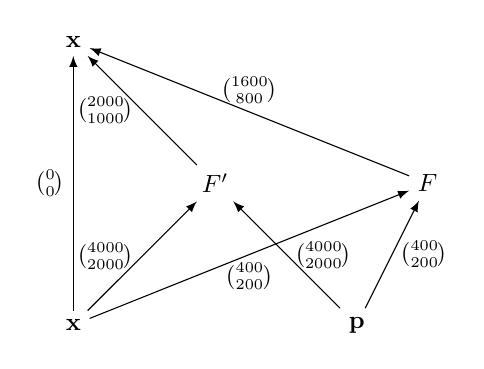
\begin{tikzpicture}[scale=.9, transform shape]
\begin{pgfscope}
%  \tikzstyle{every node}=[draw,circle]
  \node (-1) at (0,0) {$\X$};
  \node (0) at (4,0) {$\P$};
  \node (1) at (2,2) {$F'$};
  \node (2) at (5,2) {$F$};
  \node (3) at (0,4) {$\X$};
\end{pgfscope}
\begin{scope}[-latex]
 \draw (-1) -- (1) node[midway,left] {\footnotesize $\binom{4000}{2000}$};
 \draw (0) -- (1) node[midway,right] {\footnotesize $\binom{4000}{2000}$};
 \draw (-1) -- (2) node[midway,below] {\footnotesize $\binom{400}{200}$};
 \draw (0) -- (2) node[midway,right] {\footnotesize $\binom{400}{200}$};
 \draw (-1) -- (3) node[midway,left] {\footnotesize $\binom{0}{0}$};
 \draw (1) -- (3) node[midway,left] {\footnotesize $\binom{2000}{1000}$};
 \draw (2) -- (3) node[midway,above] {\footnotesize $\binom{1600}{800}$};
\end{scope}
\end{tikzpicture}
\footnotesize
$$
n=m=10
$$
	\end{minipage}
\end{frame}

\section{Conclusion and Outlook}

\begin{frame}
\frametitle{Conclusion and Outlook}
\vfill
\vfill
	\begin{center}
		\large
		\textcolor{rwth-blue}{Associativity of the chain rule matters!}
	\end{center}
\vfill
\vfill
	Work in progress:
\vfill
	\begin{itemize}
		\item Sparse compression techniques for matrix-free Jacobian chaining
		\item Automatic segmentation of (dco/c++) tape
		\item AD mission planning and control
	\end{itemize}
\vfill
\vfill
\end{frame}

\begin{frame}[allowframebreaks]
\frametitle{References}
\footnotesize
\begin{thebibliography}{10}
\bibitem{Griewank2008EDP}
	{\sc A.~Griewank and A.~Walther}, {\em Evaluating Derivatives. Principles and Techniques of Algorthmic Differentiation} (2nd ed.), SIAM, 2008,
\bibitem{Griewank1991OtC}
{\sc A.~Griewank and S.~Reese}, {\em On the calculation of {J}acobian matrices
  by the {M}arkowitz rule}, AD1991, pp.~126--135, SIAM, 1991,
\bibitem{Griewank2003AJa}
{\sc A.~Griewank and U.~N.}, {\em Accumulating {J}acobians as chained
  sparse matrix products}, Math. Prog., 95, pp.~555--571, 2003.
\bibitem{Naumann2002Etf}
{\sc U. N.}, {\em Elimination techniques for cheap Jacobians}, AD2000, pp.~247--253, Springer, 2002,
\bibitem{Naumann2020Osm}
		{\sc U.~N.}, {\em On sparse matrix chain products},
 SIAM Workshop on Combinatorial Scientific Computing, pp.~118--127, 2020.
\bibitem{Naumann2023ETf}
{\sc U.~N., E.~Schneidereit, S.~Märtens, and M.~Towara}, {\em Elimination
  techniques for algorithmic differentiation revisited}, SIAM Conference on
  Applied and Computational Discrete Algorithms (ACDA23), pp.~201--212, 2023.
\bibitem{Naumann2004Oao}
{\sc U.~N.}, {\em Optimal accumulation of {J}acobian matrices by
  elimination methods on the dual computational graph}, Math. Prog., 99, 
  pp.~399--421, 2004.
\bibitem{Naumann2008OJa}
{\sc U.~N.}, {\em Optimal {J}acobian accumulation is {NP}-complete}, Math.
  Prog., 112, pp.~427--441, 2008.
\bibitem{Naumann2008DRi}
{\sc U.~N.}, {\em {DAG} Reversal is {NP}-complete}, J. Discr. Alg.
  7, pp.~402--410, 2009.
\bibitem{Naumann2008CTR}
{\sc U.~N.}, {\em Call Tree Reversal is {NP}-complete},  AD2008, pp.~13--22, Springer, 2008,
\bibitem{Naumann2023Ano}
{\sc U.~N.}, {\em A note on the computational complexity of chain rule
  differentiation}, Optim. Methods Softw., Online, 2023.
\bibitem{Naumann2023HCB}
	{\sc U.~N. and S. Burela}, {\em Hessian Chain Bracketing}, J. Comb., 14(4), pp.~539--558, 2023.
\bibitem{Towara2021Daa}
	{\sc M.~Towara, J.~Lotz and U.~N.}, {\em Discrete adjoint approaches for CHT applications in OpenFOAM}, Advances in Evolutionary and Deterministic Methods for Design, Optimization and Control in Engineering and Science, pp.~163--178, Springer, 2021.
\end{thebibliography}
\end{frame}

\end{document}
